% !TEX root = master_thesis.tex
\chapter{Event selection}
The determination of polarization observables needs to be completed for particular reactions (cf. chapter \ref{chap:intro}), such as the photoproduction of e.g. a single $\eta'$ meson. However, the recorded events  contain data from the decay products of all possible final states in addition to combinatorical background. Thus, event candidates for the desired reaction have to be extracted before they are considered for further analysis. Table \ref{tab:etap} shows the five most probable decay modes of the $\eta'$ meson. Three of these result in final states which only contain photons and are thus reliably measurable with the CBELSA/TAPS experiment. Only the $\eta'\to\gamma\gamma$ decay channel was considered for further analysis; the $\omega\gamma$ channel provides negligible statistics and considering the acceptance of detecting six photons in the final state, the expected yield of the $\eta'\to\gamma\gamma$ decays should be roughly equal to the $\eta'\to\pi^0\pi^0\eta\to6\gamma$ final state \cite{farah}. Offering a cleaner, three-particle final state, the $\eta'\to\gamma\gamma$ was then favored in the course of this thesis.    
\begin{table}[htbp]
	\centering
	\begin{tabular}{cccc}
		\toprule
		\multicolumn{3}{c}{Decay mode}&Branching ratio\\
		\hline
		$\pi^+\pi^-\eta$&&&42.6\%\\
		$\rho^0\gamma$&$\to$&$\pi^+\pi^-\gamma$ &28.9\% (28.9\%)\\
	$\pi^0\pi^0\eta$&$\to$&$6\gamma$ & 22.8\% (8.8\%)\\
		$\omega\gamma$ &$\to$&$ \pi^+\pi^-\pi^0\gamma/\pi^0\gamma\gamma$&2.52\% (2.2\%/0.21\%)\\
	$\gamma\gamma$&&&2.3\%\\

		\bottomrule
	\end{tabular}
\caption{The five most probable decay modes of the $\eta'$ meson. The most probable further decay with according branching ratio is shown in brackets.\cite{pdg}}
\label{tab:etap}
\end{table}

\noindent The process of \emph{event selection} for the reaction $\gamma p \to p\eta'\to p\gamma\gamma$ is outlined in the following chapter. Note that in this thesis the analysis of data from $\eta$-photoproduction starts with this process already completed, which is described in detail in reference \cite{farahphd}.

\section{Preselection and charge cut}
Events are generally classified depending on the number of particle energy deposits (PED). If the complete four-momenta of three final state particles are measured, they are referred to as 3PED events. Low energy protons however may either be only detected in the scintillators of the inner, forward or MiniTAPS detector -- giving only directional information (2.5 PED) -- or lost entirely (2 PED). Only 2.5PED and 3PED events were analyzed since the additional background contributions from 2PED events exceeded the additional signal contributions. It is worth noting that 3PED events are significantly dominant for $\eta'\to\gamma\gamma$ reactions; the production threshold for $\eta'$ mesons is $E_\gamma=\SI{1447}{\mega\eV}$, such that the recoil proton will likely be detected. Figure \ref{fig:PEDs} shows the distribution of the different event classes for $\eta'\to\gamma\gamma$ production in \textsc{Monte Carlo} data, with a clear preference towards 3PED events.

\begin{figure}[htbp]
	\centering
	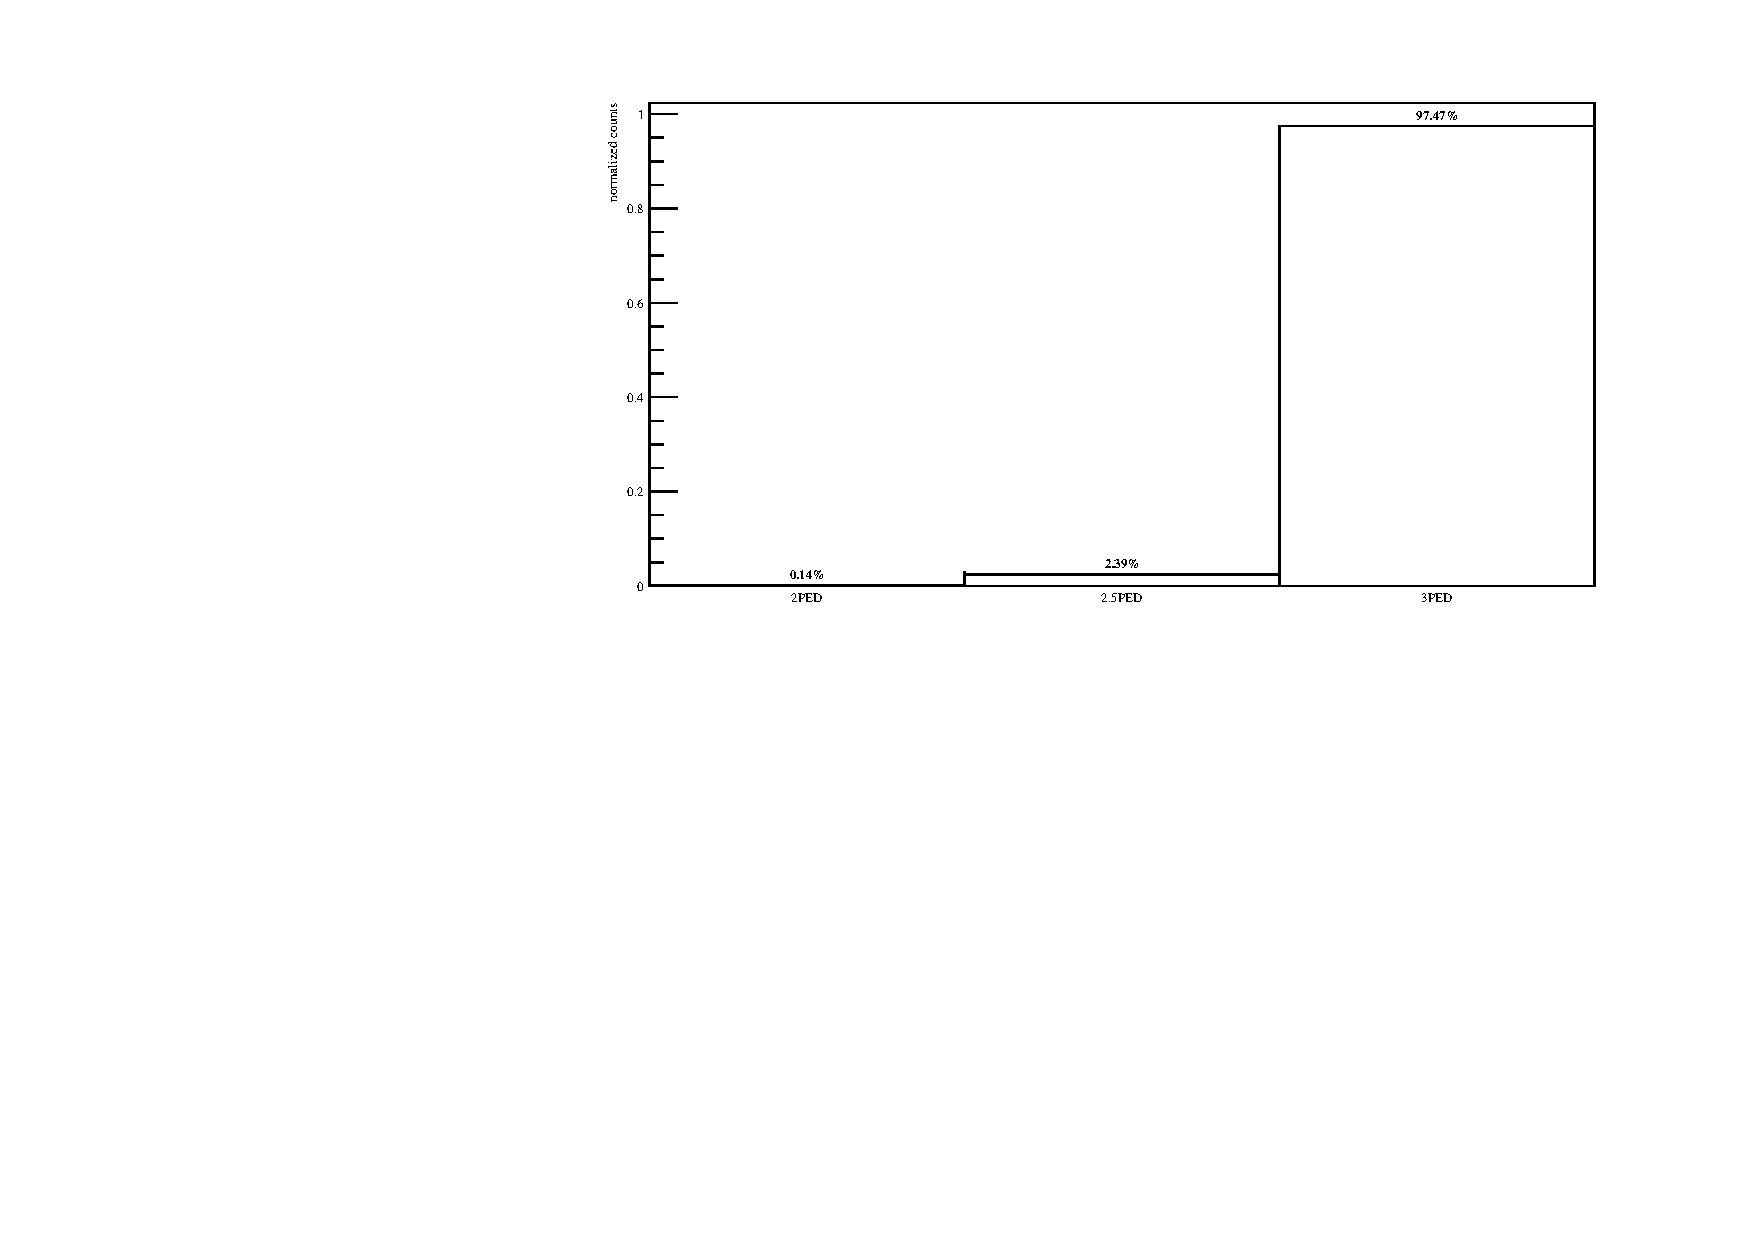
\includegraphics[width=\linewidth]{../figs/hydrogen/PEDs.pdf}
	\caption{Distribution of event classes in $\eta'\to\gamma\gamma$ production}
	\label{fig:PEDs}
\end{figure}




 To further improve the signal to background ratio, the charge information of the final state particles was utilized in the next step. In particular, to select  $\eta'\to\gamma\gamma$ reactions, one charged and two uncharged particles in the final state were demanded. 

\section{Time of particles}
Due to its high count rate the tagging system (see section \ref{subsec:tag}) will not only record beam photons which produce the detectable final state particles, but also several uncorrelated ones. To select only beam photons which will induce a photoproduction process the time information of the detected particles is used. It is shown in figure \ref{fig:time} for all particles involved in 2.5PED and 3PED events of $\eta'$ photoproduction. 
\begin{figure}[htbp]
	\centering
	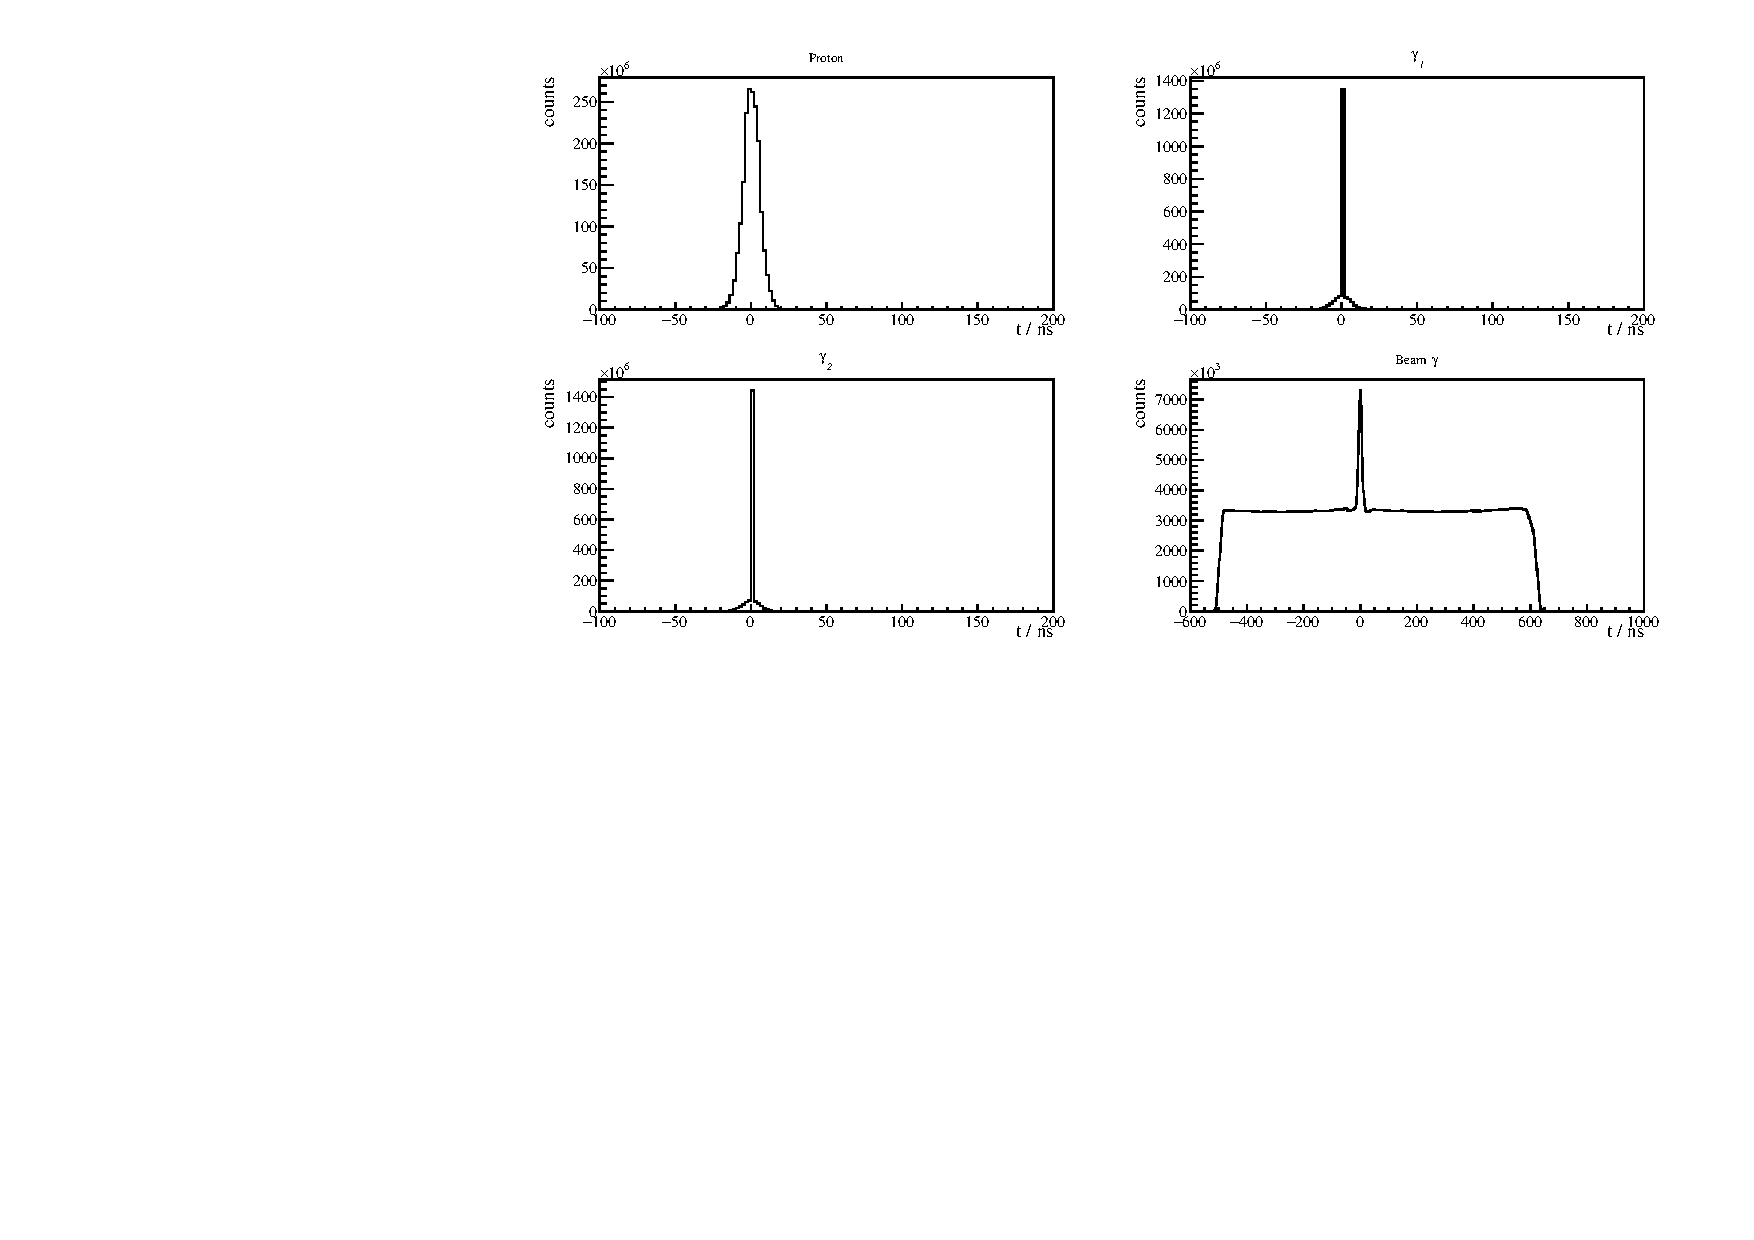
\includegraphics[width=\linewidth]{../figs/hydrogen/time/times.pdf}
	\caption{Time information of all final state particles and the beam photon for 3PED $\eta'$ production}
	\label{fig:time}
\end{figure} 
In all cases prompt peaks centered around \SI{0}{\nano\s} (the trigger time) are visible. Since the final state photons move with velocity $c$ their timing information does not underlie fluctuations, as is the case for the final state proton on the contrary. The tagged, uncorrelated beam photons are visible as flat background underneath the prompt peak in the time of the beam photon. Naturally, only coincident events may be referred to  as $\eta'$ candidates for the further analysis and thus only events with time information of at least one final state particle are kept. Photons need to be detected in the MiniTAPS or forward
detector to acquire time information. To determine coincidence it is convenient to define the \emph{reaction time} 
\begin{equation}
	t_\text{reaction}=\begin{cases}
		t_\text{beam}-t_\text{meson} & \text{ meson time exists}\\
		t_\text{beam}-t_\text{recoil} & \text{ meson time does not exist},
	\end{cases}
\end{equation}
where the meson time $t_\text{meson}$ is appointed either the averaged time of both decay photons or the time of a single photon if only one photon has time information. $t_\text{beam}$ and $t_\text{recoil}$ are the time of the beam photon and recoil proton, respectively. Figure \ref{fig:time_r} shows the reaction time for 2.5PED and 3PED events; a clear prompt peak centred at 0 is visible, the colored area indicates the chosen range of $t_\text{reaction}\in[-8,5]\si{\nano\s}$. However, this cut still contains random time background underneath the prompt peak. This may be accounted for by \emph{sideband substraction}, assuming the background is flat. All events residing in the prompt peak with $t_r\in[-8,5]\si{\nano\s}$ will be assigned a weight of $w_p=+1$ while sideband events with $t_r\in[-200,-100]\si{\nano\s}\lor t_r\in[100,200]\si{\nano\s}$ will be assigned a weight of $w_s=-\frac{13}{200}$. Any histogram $N$ that is filled in the following will then consist of prompt peak events $N_\text{prompt}$ and sideband events $N_\text{sideband}$ $$N=N_\text{prompt}+w_s\cdot N_\text{sideband},$$ such that the random time background underneath the prompt peak is substracted. In addition, the time difference between meson and proton and between the two photons is demanded to be within $[-10,10]\si{\nano\s}$. All described cuts to the data, including the sideband substraction are referred to as the \emph{time cut} in the following.

\begin{figure}[htbp]
	\centering
	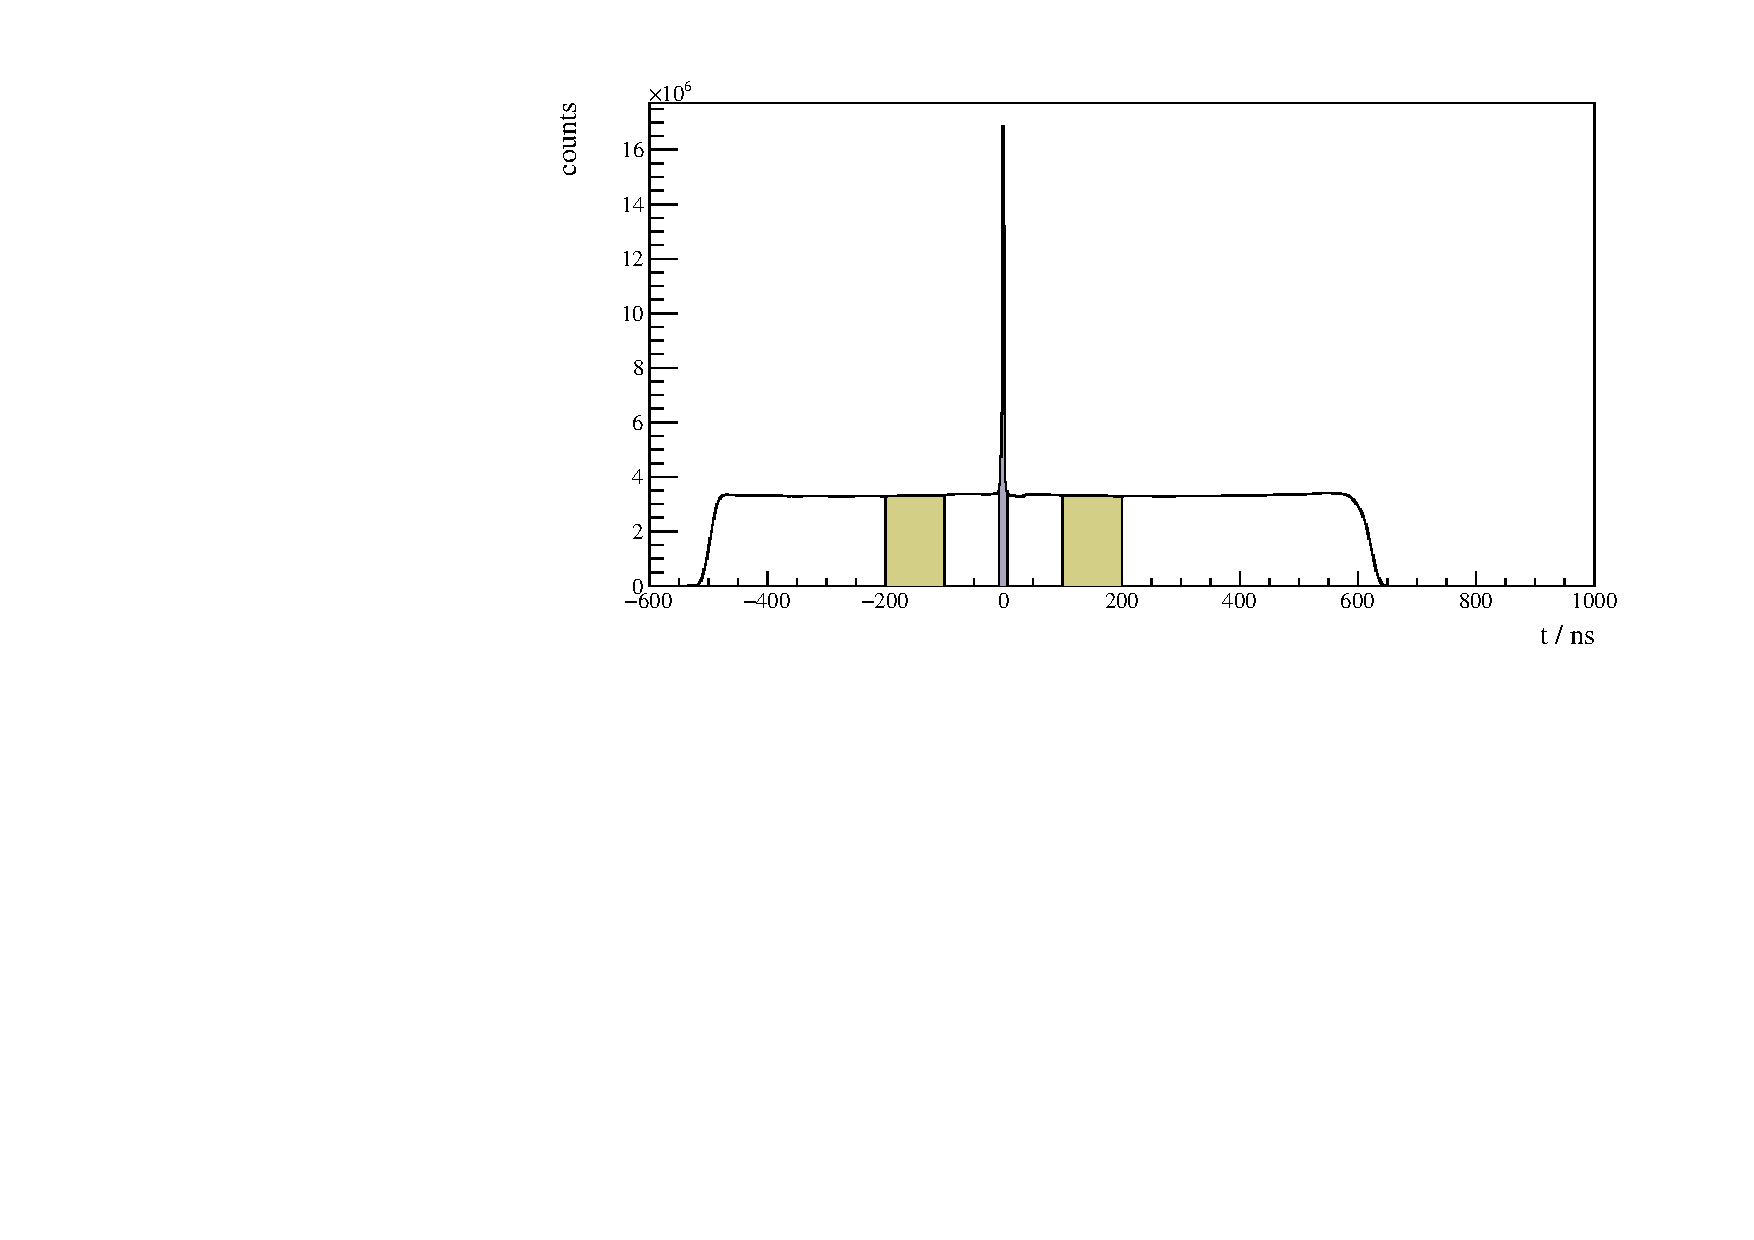
\includegraphics[width=\linewidth]{../figs/hydrogen/time/reaction_time.pdf}
	\caption{Reaction time $t_r$ for 3PED $\eta'$ production}
	\label{fig:time_r}
\end{figure} 

\section{Kinematic constraints}
Up until now mainly combinatorical background was discussed. However one can derive kinematical constraints from energy and momentum conservation to exclusively select the desired reaction. The derivation is discussed first, followed by the determination of the derived cut conditions.
\subsection{Derivation of cut conditions}
After charge and time cut, additional cuts can be derived from energy and momentum conservation. Let $p_\text{beam}$ and $p_p$ be the four momenta of the initial state beam photon and proton, respectively. Then \begin{equation}
	p_\text{beam}+p_p=p_\text{recoil}+p_\text{meson}
	\label{eq:kin}
\end{equation}
holds, with $p_\text{recoil}$ being the momentum of the recoiling proton and $p_\text{meson}$ the meson momentum.
\subsubsection{Coplanarity}
In the initial state there is vanishing transversal momentum $p_{xy}$ since the target protons are at rest and the beam photon impinges in $z$-direction. Naturally this transversal momentum has to vanish in the final state as well, such that \begin{equation}
	\mathcal{P}_{xy} \left[p_\text{recoil}+p_\text{meson}\right]=0,
	\label{eq:copl}
\end{equation}
where $\mathcal{P}_{xy}$ is the projection operator to the transversal plane. Equation \eqref{eq:copl} is valid if and only if meson and proton lie back to back (coplanar) in the $x$-$y$ plane, which is quantified by the difference of their azimuthal angles $\phi_\text{meson}$ and $\phi_\text{recoil}$ being $\SI{180}{\degree}$ in the laboratory-frame
\begin{equation}
	\Delta\phi:=\phi_\text{meson}^\text{LAB}-\phi_\text{recoil}^\text{LAB}\overset{!}{=}\SI{180}{\degree}.
\end{equation}
\subsubsection{Polar angle difference}
If all initial and final state momenta are measured, the reaction described by equation \eqref{eq:kin} is \emph{overdetermined}, such that one final state particle can be treated as a "missing particle" $X$ with momentum $p_X$: 
\begin{equation}
	p_X=p_\text{beam}+p_p-p_\text{meson}.
	\label{eq:polangle}
\end{equation}
One can then use 
\begin{equation}
\Delta\theta:=\theta_{p_X}^\text{LAB}-\theta_{p_\text{recoil}}^\text{LAB}\overset{!}{=}0
\label{eq:polarangle}	
\end{equation}
as a further constraint to the data.
\subsubsection{Missing mass}
The previously described angular cuts are only applicable if all final state particles have been detected. Independently of the detection of the recoil proton the mass of the missing particle $m_X^2=p_X^2$ can be determined and compared with the proton mass of $m_p=\SI{938.27}{\mega\eV}$ \cite{pdg}. From equation \eqref{eq:polangle} it follows that \begin{equation}
	m_X=\sqrt{(E_\gamma+m_p-E_\text{meson})^2-p_{x,\text{meson}}^2-p_{y,\text{meson}}^2-(E_\gamma-p_{z,\text{meson}})^2}.
	\label{eq:mism}
\end{equation}
\subsubsection{Invariant mass}
The measurement of the invariant mass of the two final state photons does also not require the measurement of the recoil proton. The knowledge of both four-momenta suffices, since \begin{equation}
	m_\text{meson}=\sqrt{p_\text{meson}^2}=\sqrt{(p_{\gamma_1}+p_{\gamma_2})^2}=\sqrt{2E_{\gamma_1}E_{\gamma_2}(1-\cos\alpha_{\gamma_1\gamma_2})},
\label{eq:invm}
\end{equation}
where $E_{\gamma_i}$ are the measured photon energies and $\alpha_{\gamma_1\gamma_2}$ is the angle spanned by the two photon momenta. To select only $\eta'$ candidates $m_\text{meson}=m_{\eta'}=\SI{957.78}{\mega\eV}$ is demanded. Remarkably, the cut on the invariant mass of the final state photons is the only one to uniquely select $\eta'$ production candidates so far. All other cuts apply similarly to arbitrary meson photoproduction.
\subsection{Determination of cut ranges}
The constraints described in the previous section must not be understood as strict equalities, cf. equations \eqref{eq:copl},\eqref{eq:polarangle},\eqref{eq:mism} and \eqref{eq:invm}. The quantities of interest will rather describe distributions around the desired value, such that confidence intervals may be extracted by fitting to said distributions. This is done iteratively:

Let $\mathcal{C}^\chi_{\mathcal{I}}$ be the cut operator that restrains the data $\mathcal{D}$ such that the (generic) cut variable $$\chi\in\{\Delta\theta,\Delta\phi,m_X,m_\text{meson}\}$$ lies in the interval $\mathcal{I}\subseteq\mathbb{R}$, such that 
\begin{equation}
	\mathcal{C}_{\mathcal{I}}^\chi:\mathcal{D}\mapsto\mathcal{D}_{\chi\in\mathcal{I}} .
\end{equation}
\begin{enumerate}
	\item After a first inspection of the data, initial guesses for the intervals $\mathcal{I},\mathcal{J},\mathcal{K},\mathcal{L}$ corresponding to the quantities $\Delta\theta,\Delta\phi,m_X,m_\text{meson}$ respectively are made.
	\item Having established estimates for the cut ranges, new ones are estimated by investigating the distribution of one cut variable obtained from the data while all other cut variables are constrained to the previously determined intervals. For example 
	$$\Delta\theta\left(\mathcal{C}_\mathcal{J}^{\Delta\phi}\mathcal{C}_\mathcal{K}^{m_X}\mathcal{C}_\mathcal{L}^{m_\text{meson}}\mathcal{D}\right)\sim \text{normal}(\mu,\sigma),$$
	where $\mu\approx0$. This is done (with some adjustments to the fit function) for each cut variable. The parameters of the gaussian are determined from a $\chi^2$ fit and used to assign new cut ranges. Simultaneously, Monte-Carlo (MC) data of relevant final states are fitted to match the measured values bin-wise. This is done on the one hand to check consistency between measured and MC data and on the other hand used to determine contributing background reactions. Depicted in table \ref{tab:mc} are the considered reactions which spectra are fitted to the data.
	\begin{table}
		\begin{tabular}{c}
			$\pi^0$ \\
		\end{tabular}
	\end{table}
	
	 Since the invariant mass spectrum features rich contributions from many final states, it is difficult to describe by a (sum of) gaussian function(s), especially considering the background contributions. Thus, for the invariant mass the cut ranges are obtained from gaussian fits to the scaled MC data of the $\eta'$ final state. Table \ref{tab:cuts} shows which fit function and cut range was used for each cut variable. In addition, it shows if the cut ranges were determined from MC or measured data.
	\begin{table}[htbp]
		\centering
		\begin{tabular}{cccc}
			\toprule
			cut variable & fit function & interval range & obtained from\\
			\hline
			$\Delta\theta$&\textsc{Gauss}&$\mathcal{I}'=[\mu-3\sigma,\mu+3\sigma]$&data points\\
			$\Delta\phi$&\textsc{Gauss}&$\mathcal{J}'=[\mu-3\sigma,\mu+3\sigma]$&data points\\
			$m_X$&\textsc{Novosibirsk} \cite{nov}&$\mathcal{K}'=[\mu-2\sigma,\mu+2\sigma]$&data points\\
			$m_\text{meson}$&\textsc{Gauss}&$\mathcal{L}'=[\mu-2\sigma,\mu+2\sigma]$&MC data\\
			
			\bottomrule
		\end{tabular}
		\caption{Fit functions and cut ranges for each variable}
		\label{tab:cuts}
	\end{table}
\item The newly obtained intervals $\mathcal{I}',\mathcal{J}',\mathcal{K}',\mathcal{L}'$ serve again as input for step 2. This is repeated until a certain convergence is reached, which is usually the case after a two or three iterations.
\end{enumerate}
 Since the cut ranges may vary depending on beam energy and meson direction, they are determined in bins of the beam energy and the CMS polar angle of the meson $$(E_\gamma,\cos\theta_{\eta'}^\text{CMS}).$$ Respecting the $\eta'$ final state statistics, a binning of $\Delta E_\gamma=\SI{100}{\mega\eV}$ and $\Delta\cos\theta_{\eta'}^\text{CMS}=1/3$ was chosen, spanning the energy range of \SIrange{1500}{1800}{\mega\eV}. The theoretically accessible lower limit in the beam energy is provided by the production threshold of $\eta' $ mesons at \SI{1447}{\mega\eV} \cite{pdg}. Yet, the binning has to comply with the upper beam energy limit which is bounded from above \footnote{Significantly beyond the coherent edge, the systematic error for the beam polarization  degree gets too large ($>10\%$)} by the position of the coherent edge of the beamtime. It is given by \SI{1700}{\mega\eV} and \SI{1800}{\mega\eV} for the July/August and September/October beam times, respectively. If one were to include the production threshold into the analyzed range using the same binning, more background than $\eta'$ events are collected from \SIrange{1400}{1500}{\mega\eV}, hence the chosen binning starts at \SI{1500}{MeV}.
 
 \subsubsection{Coplanarity}
 Figure \ref{fig:copl} shows the coplanarity spectra for the energy bin $\SI{1500}{\mega\eV}\leq E_\gamma<\SI{1600}{\mega\eV}$ and all angular bins. The data points are visualized by the open circles with error bars, while the black solid histogram is a fit of $\eta'\to\gamma\gamma$ MC. As expected, a clear peak is visible at $\Delta\phi=\SI{180}{\degree}$, which shows only slight dependence on beam energy and meson direction. A $3\sigma$ interval obtained from a gaussian fit is indicated by the dashed red lines. Note that only MC spectra of the $\eta'$ final state were fitted to the data since the coplanarity gives little reference points for other final states that may contribute. 
   \begin{figure}[htbp]
 	\centering
 	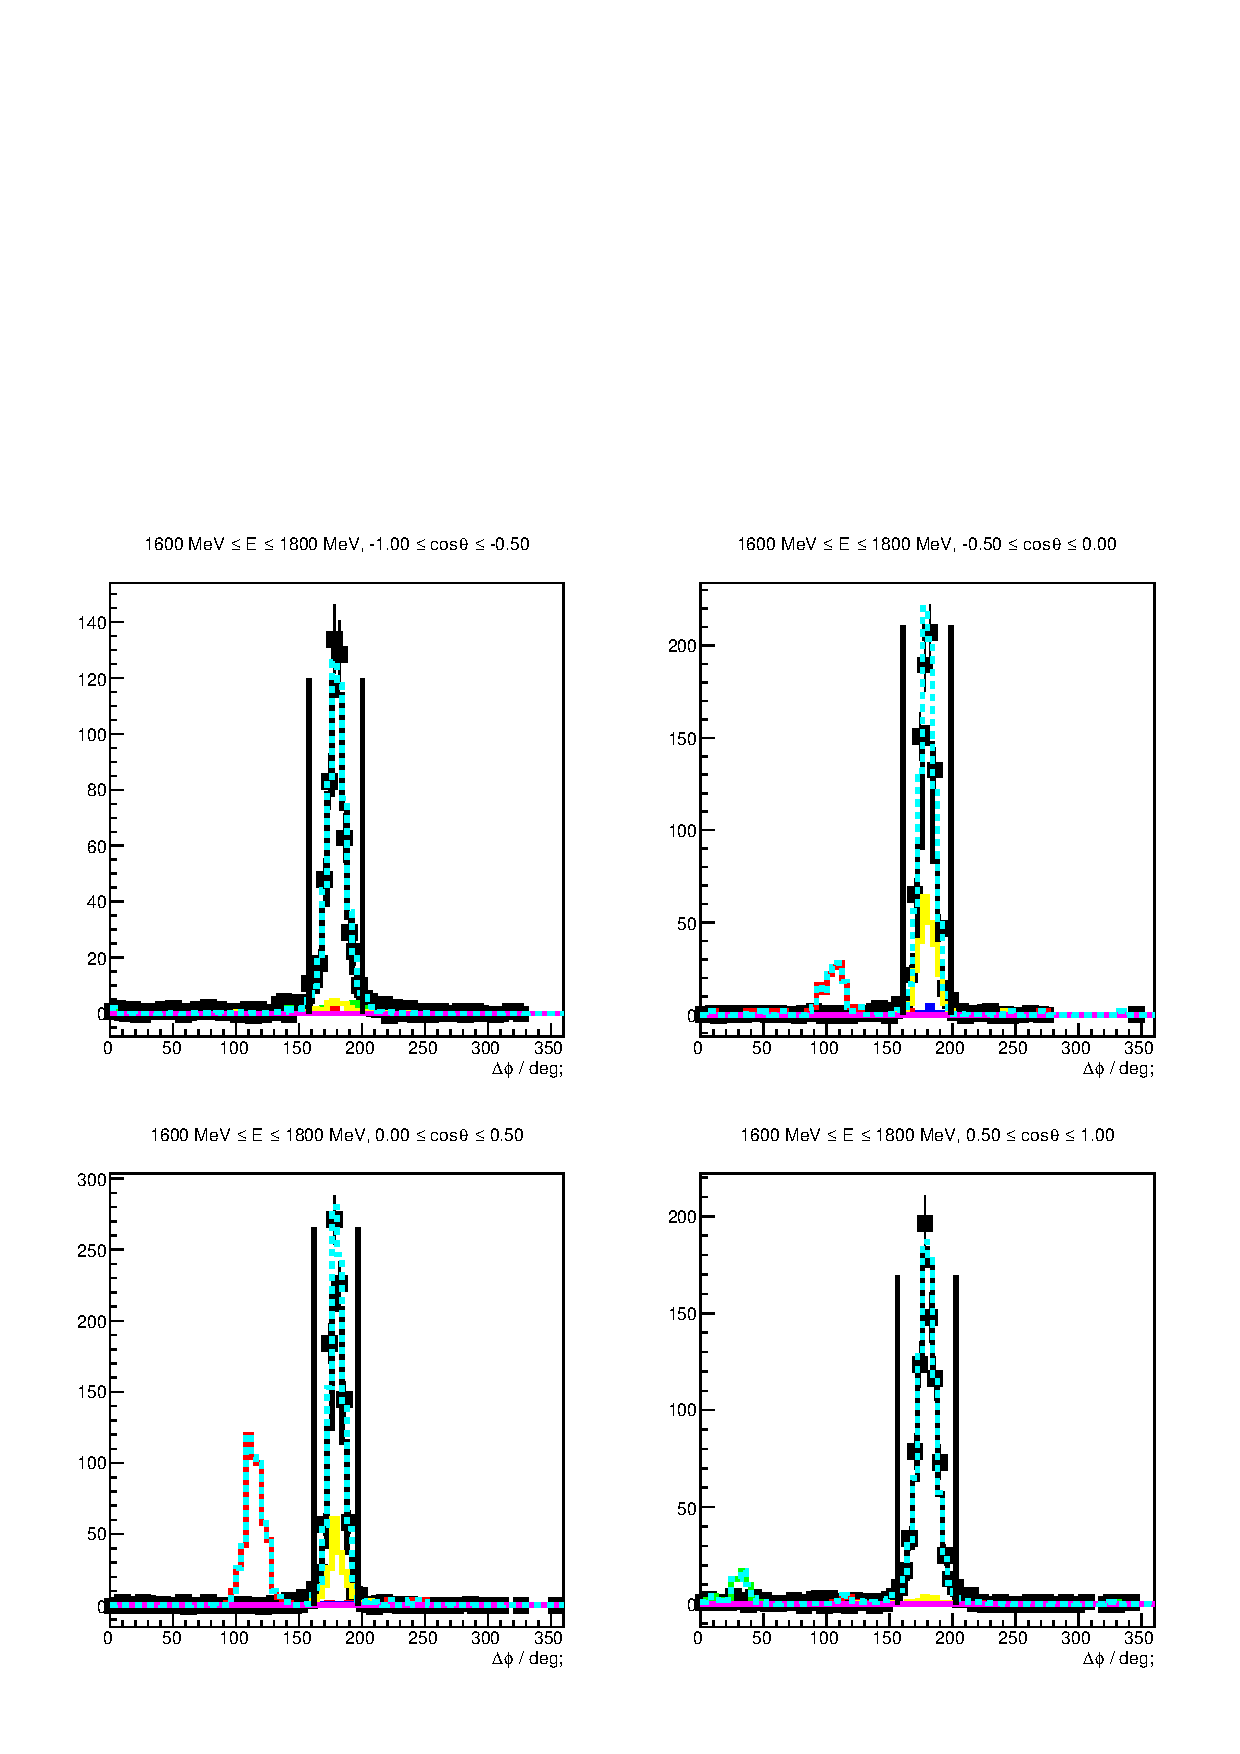
\includegraphics[width=\linewidth]{../figs/hydrogen/bin_cuts/phicut_ebin1.pdf}
 	\caption{Coplanarity of the $p\eta'$ final state with all other cuts applied. The vertical dashed lines show the cut ranges obtained from a gaussian fit to the data (open circles). The solid black histograms represent fitted MC data of $\eta'\to\gamma\gamma$}
 	\label{fig:copl}
 \end{figure}
 \subsubsection{Polar angle difference}
 Since the meson direction correlates with the detector(s) the final state photons hit, the polar angle difference depicts a clear directional dependence as can be seen in figure \ref{fig:pol} for the energy bin $\SI{1500}{\mega\eV}\leq E_\gamma<\SI{1600}{\mega\eV}$ and all angular bins. In the CMS frame, meson and proton are emitted back to back. Thus, if the meson is emitted in backward direction ($\cos\theta_{\eta'}^\text{CMS}\sim -1$), the proton will be detected either in the forward or MiniTAPS detector, which have a better angular resolution than the Crystal Barrel calorimeter, leading to narrower distributions of $\Delta\theta$. The determined cut ranges are $3\sigma$ intervals obtained from a gaussian fit to the data and are indicated by the red dashed lines. As before, no other than $\eta'$ MC are fitted to the spectra.
  \begin{figure}[htbp]
 	\centering
 	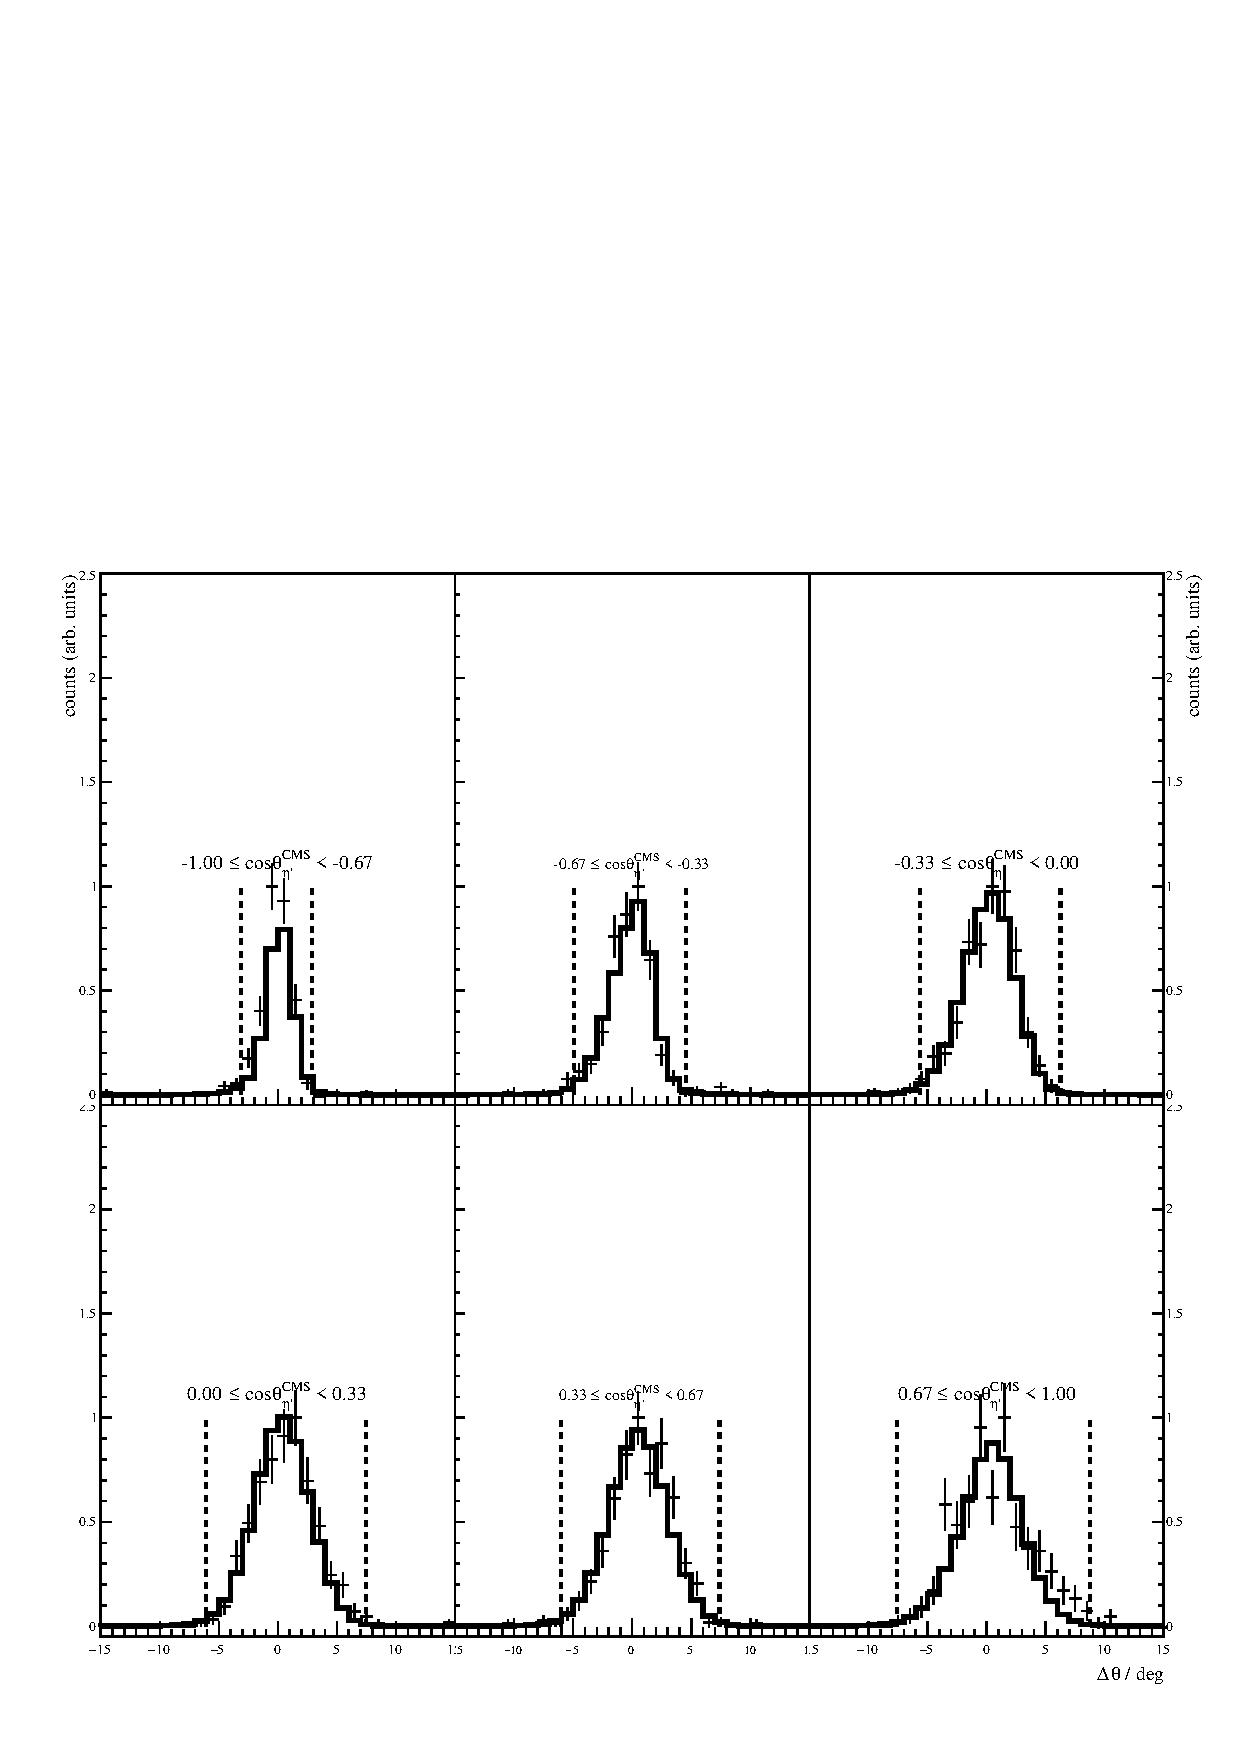
\includegraphics[width=\linewidth]{../figs/hydrogen/bin_cuts/thetacut_ebin1.pdf}
 	\caption{Polar angle difference of the $p\eta'$ final state with all other cuts applied. The vertical dashed lines show the cut ranges obtained from a gaussian fit to the data (open circles). The solid black histograms represent fitted MC data of $\eta'\to\gamma\gamma$}
 	\label{fig:pol}
 \end{figure}
 \subsubsection{Missing mass}
 The missing mass spectra allow a first investigation of possible background reactions that pass event selection. For all angular bins of the first energy bin the missing mass is shown in figure \ref{fig:mism}; again, the open circles are the data points with corresponding statistical error bars. The solid colored histograms are fitted MC spectra of different possible background contributions while the black histogram is the signal contribution of $\eta'\to\gamma\gamma$ photoproduction. The turquoise histogram is the sum of all MC histograms. Generally, most of the data can be described by the $\eta'$ MC alone, but especially towards higher masses (and higher beam energies) background contributions extend the missing mass peak as flat background. These are reactions where the meson mass $m_\text{meson}^2=E_\text{meson}^2-\vec{p}_\text{meson}^2$ is smaller than the $\eta'$ mass, resulting in larger values for the missing mass. Judging from the fit to the missing mass, $2\pi^0$ and/or $\pi^0\eta$ photoproduction may describe the background as both show similar shapes. Better conclusions can be drawn from the invariant mass spectra as is discussed in the following section \ref{sec:bkg}. The cut ranges for the missing mass are obtained from a \textsc{Novosibirsk} fit to the data since the missing mass distribution is slightly asymmetric. However, since the tail parameter is small, still a symmetric cut of $\pm2\sigma$ was chosen. It was chosen narrower than the angular cuts to collect less background reactions.
  \begin{figure}[htbp]
 	\centering
 	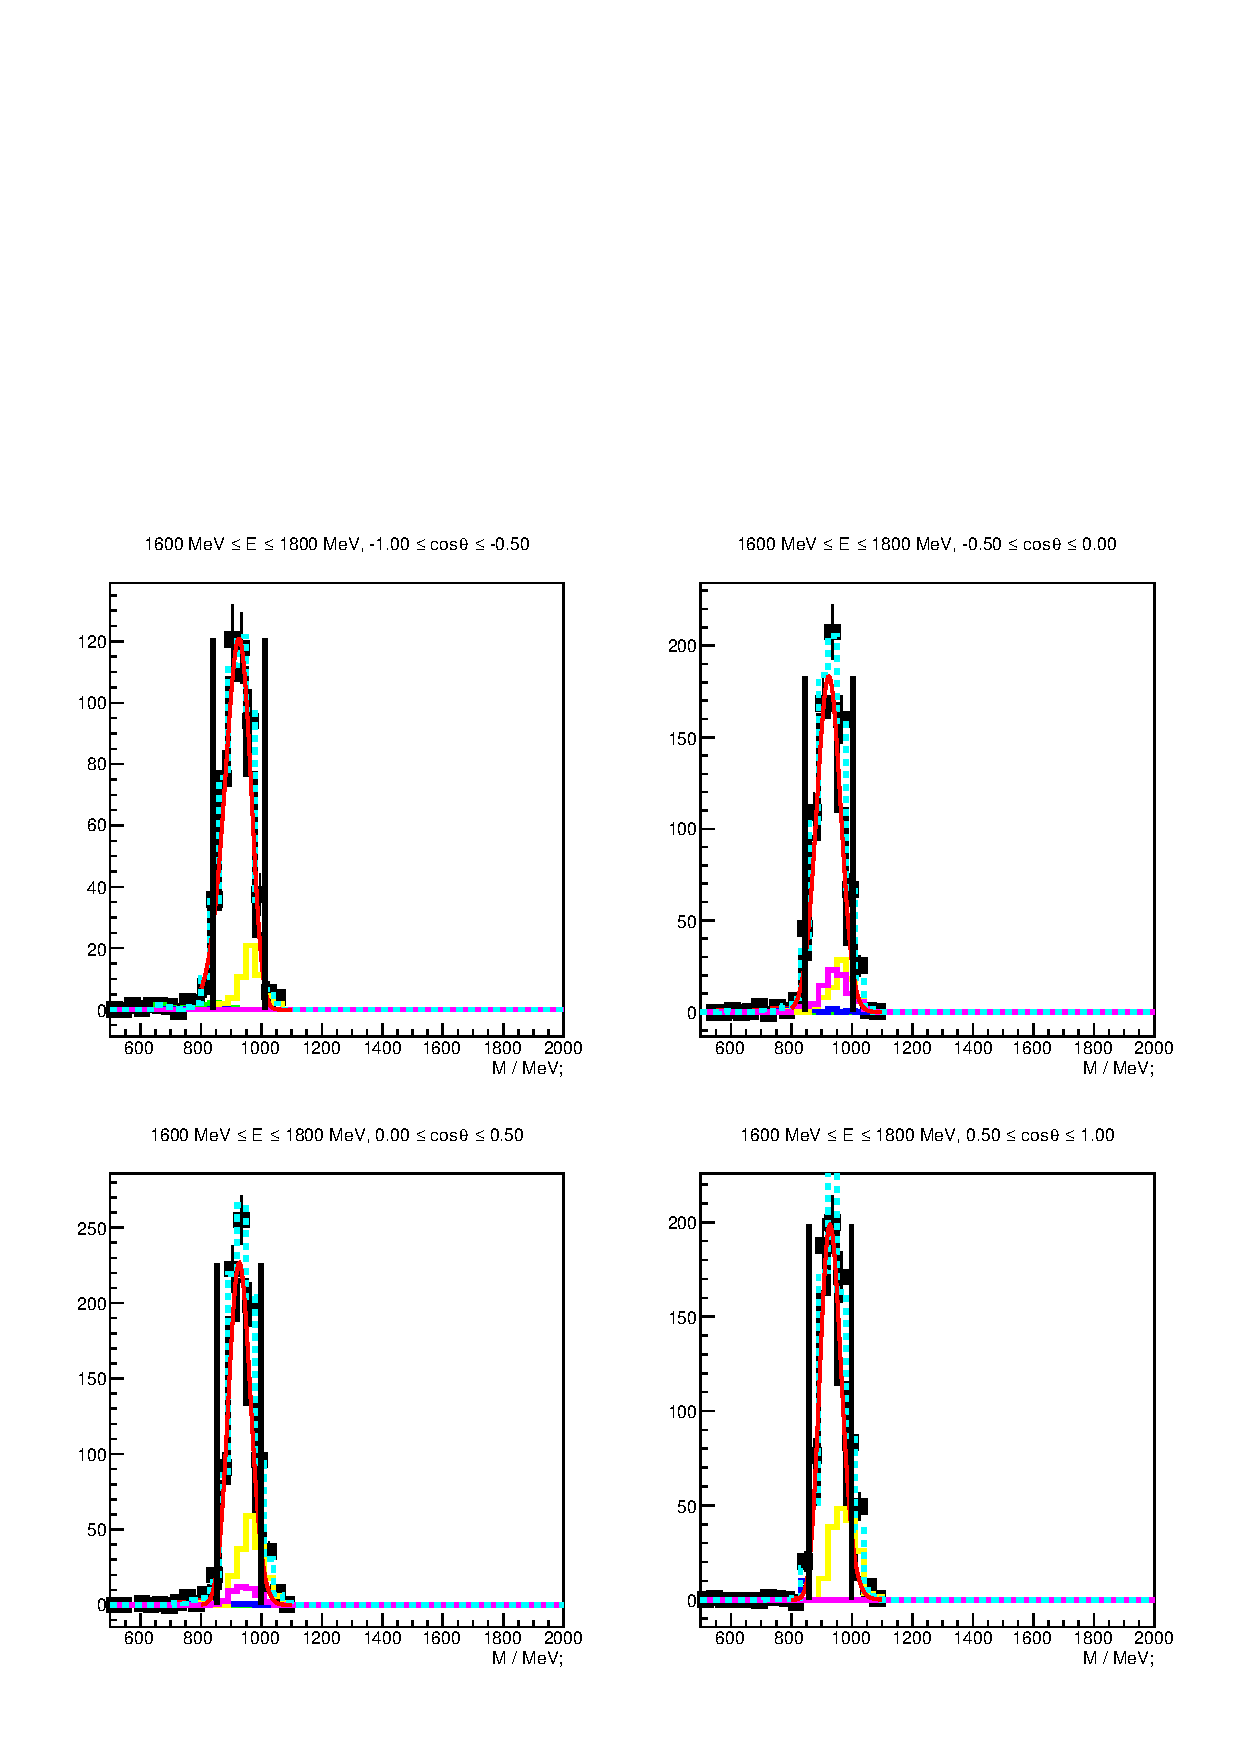
\includegraphics[width=\linewidth]{../figs/hydrogen/bin_cuts/mismcut_ebin1.pdf}
 	\caption{Missing mass of the $p\eta'$ final state with all other cuts applied. The vertical dashed lines show the cut ranges obtained from a fit to data (open circles) employing a \textsc{Novosibirsk} function. The solid colored histograms represent fitted MC data from relevant  photoproduction reactions: in black $\eta'$, in green $\pi^0$, in red $\eta$, in blue $\omega$, in yellow $2\pi^0$, magenta $\pi^0\eta$. The turquoise histogram is the sum of all MC histograms.}
 	\label{fig:mism}
 \end{figure}
 \subsubsection{Invariant mass}
 Investigating the invariant mass spectrum of the final state photons allows to illustrate the impact of the event selection so far. As has been mentioned all cuts considered up to this point apply to arbitrary meson photoproduction. This means that the invariant mass spectrum will depict peaks belonging to mesons produced in the considered beam energy range. This is shown in
 
 \begin{figure}[htbp]
 	\centering
 	\includegraphics[width=\linewidth]{imagefile}
 \end{figure}
 
 
 
 \begin{figure}[htbp]
 	\centering
 	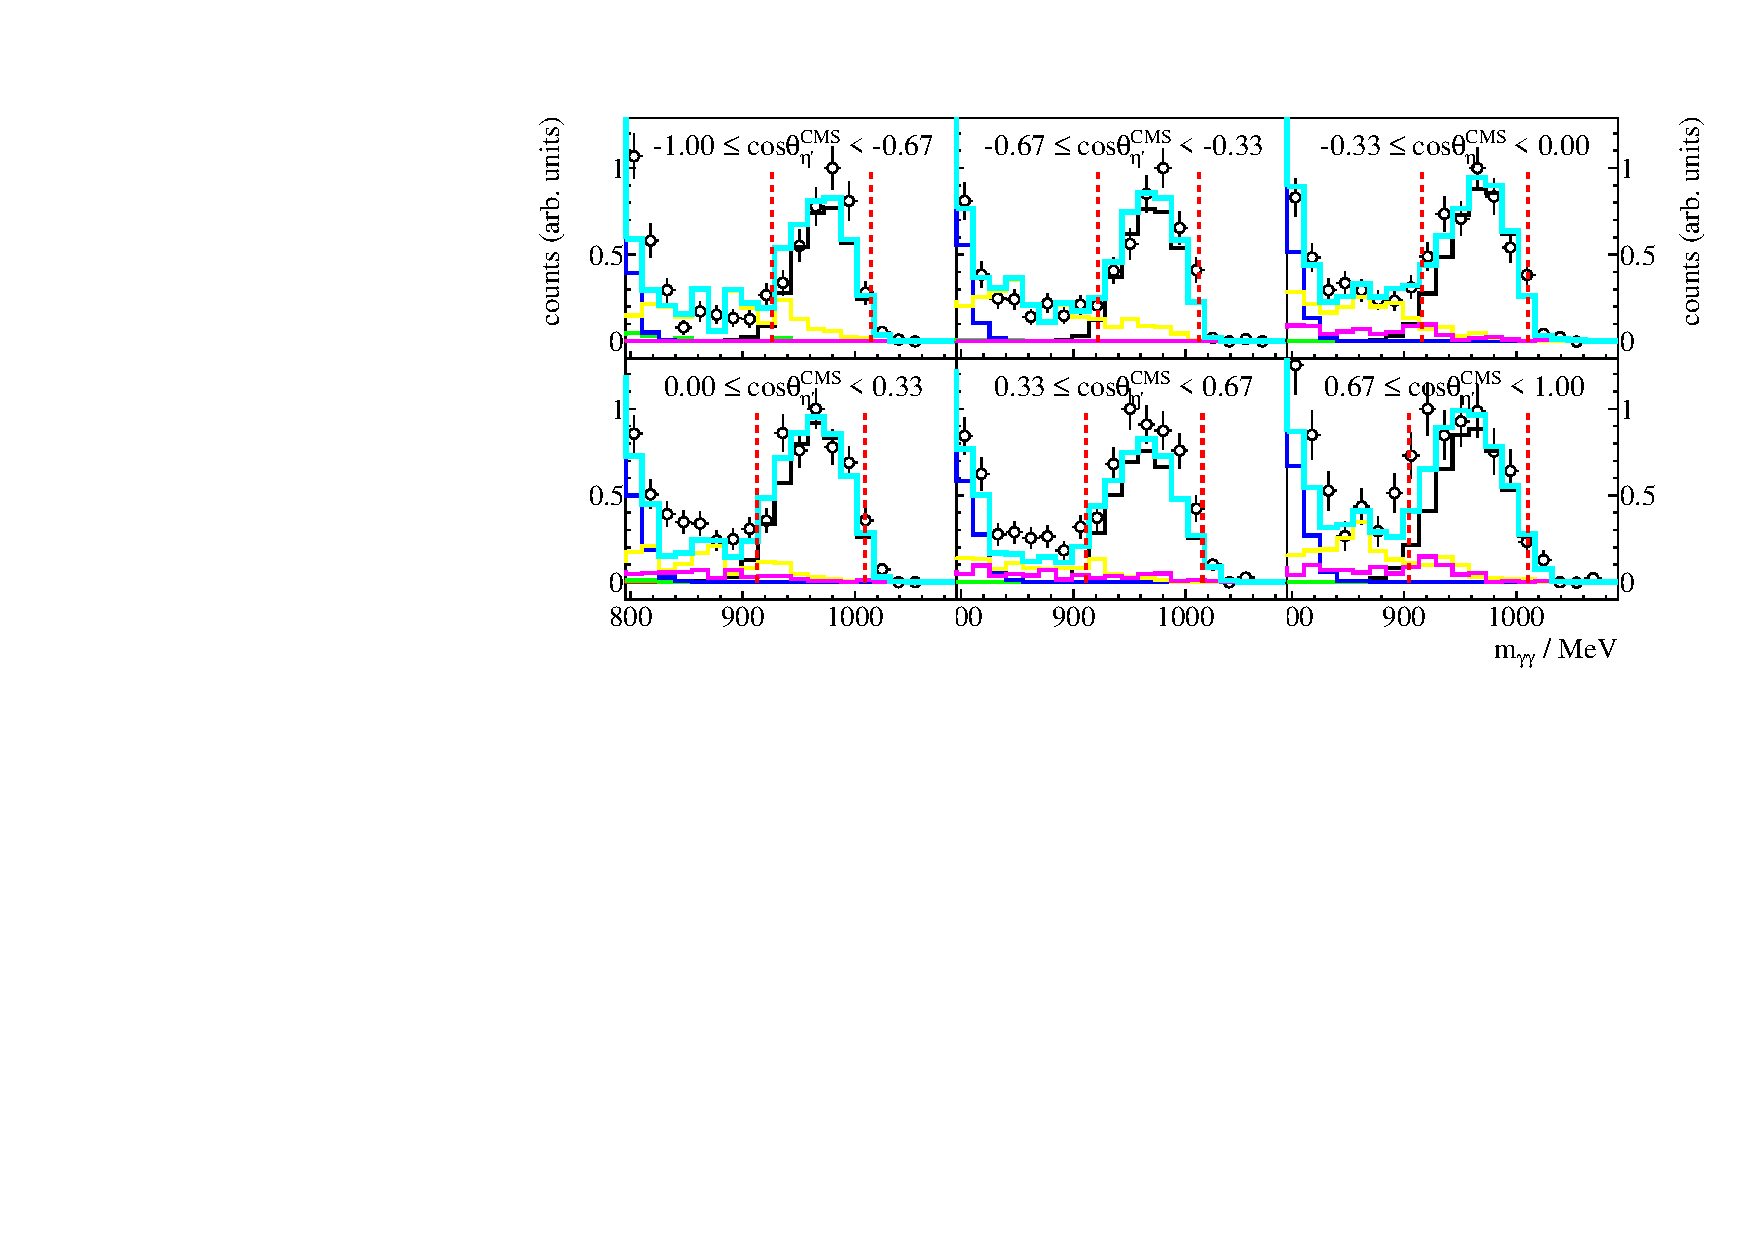
\includegraphics[width=\linewidth]{../figs/hydrogen/bin_cuts/invcut_ebin1.pdf}
 	\caption{Invariant mass of the $p\eta'$ final state with all other cuts applied. The vertical dashed lines show the cut ranges obtained from a gaussian fit to the $\eta'$ MC data (solid black histogram). The open circles represent the measured data, the solid colored histograms fitted MC data from relevant photoproduction reactions: in black $\eta'$, in green $\pi^0$, in red $\eta$, in blue $\omega$, in yellow $2\pi^0$ and in magenta $\pi^0\eta$. The turquoise histogram is the sum of all MC histograms.}
 	\label{fig:invm}
 \end{figure}
\section{Investigation of background and additional cuts} 
\label{sec:bkg}